% docs/ecfi_minipaper_trace_v2.tex
\documentclass[11pt]{article}

\usepackage[a4paper,margin=2.6cm]{geometry}
\usepackage{amsmath,amssymb}
\usepackage{booktabs}
\usepackage{graphicx}
\usepackage{hyperref}
\usepackage{enumitem}

\hypersetup{
  colorlinks=true,
  linkcolor=blue,
  citecolor=blue,
  urlcolor=blue
}

% ---- Notation helpers (avoid N vs \mathcal{N} collision) ----
\newcommand{\R}{\mathbb{R}}
\newcommand{\Neigh}{\mathcal{N}} % neighbor set
\newcommand{\nov}{\nu}          % novelty
\newcommand{\varph}{\varphi}    % prefer \varphi
\newcommand{\norm}[1]{\left\lVert #1 \right\rVert}

\title{Tracing a Minimal E-CFI Demo: Baseline Diagnostics, H$'$ Switching, and the H$''$ Plan (Heterogeneous Oscillators)}
\author{Internal mini-paper (repository trace)}
\date{\today}

\begin{document}
\maketitle

\begin{abstract}
This note documents two consecutive diagnostic cycles of a minimal Embodied Collective Free Improvisation (E-CFI) demo prototype.
The system couples (i) embodied self-assembly (join/detach and assembly graph components), (ii) event-driven oscillators with merge-triggered
phase synchronization, and (iii) a two-time-scale CFI-inspired cognitive layer (fast intention, slow objective) modulated by intrinsic signals
(novelty, boreness, load proxies).
We report (H) a baseline failure mode where both assembly and phases collapse into globally locked regimes, and (H$'$) a tuned configuration that
successfully induces switching in the assembly layer while leaving global phase coherence in an absorbing synchronized state.
We conclude by defining H$''$: introducing small heterogeneity in oscillator natural frequencies ($\omega_0$) so that coherence becomes sensitive
to detachments and reconfigurations.
\end{abstract}

\section{Prototype snapshot}
The prototype implements: (a) an assembly graph $G_A(t)$ built by slot-limited joins within radius $R_C$ and probabilistic detachments after
a dwell time $T_{\min}$, (b) oscillator phases $\varph_k(t)\in[0,1)$ with free-running drift, synchronized on component merges,
(c) a minimal CFI-inspired cognition layer with a 3D feature vector
$x_k(t)=(\deg_k(t),\ \text{cluster\_size}_k(t),\ \text{local\_coherence}_k(t))$, and (d) intrinsic signals driving objective shifts toward
independence.

\section{Baseline diagnostic cycle (H)}
Figures~\ref{fig:H_clusters}--\ref{fig:H_intrinsic} summarize the baseline run (\texttt{configs/base.yaml}, seed 0). The system rapidly collapses
into a single assembly component, and merge-triggered hard synchronization drives global phase coherence to an absorbing lock-in.

\begin{figure}[t]
  \centering
  
\includegraphics[width=0.92\linewidth]{figures/plot_clusters.png}
  \caption{\textbf{(H) Assembly regime indicators.} Rapid collapse to one connected component: $n_{\text{clusters}}(t)\to 1$ and
  mean cluster size $\to N$.}
  \label{fig:H_clusters}
\end{figure}

\begin{figure}[t]
  \centering
  
\includegraphics[width=0.92\linewidth]{figures/plot_coherence.png}
  \caption{\textbf{(H) Global phase coherence.} Coherence quickly reaches $1$ and remains locked (absorbing synchronized state).}
  \label{fig:H_coherence}
\end{figure}

\begin{figure}[t]
  \centering
  
\includegraphics[width=0.92\linewidth]{figures/plot_intrinsic.png}
  \caption{\textbf{(H) Intrinsic signals.} Novelty shows early transients; load remains high; boreness appears flat at the plotted scale
  (expected if the boreness update tends to $\mathcal{O}(\eta)$ and thresholds are not crossed).}
  \label{fig:H_intrinsic}
\end{figure}

\section{Tuned diagnostic cycle (H$'$): assembly switching without coherence switching}
Figures~\ref{fig:Hp_clusters}--\ref{fig:Hp_intrinsic} summarize the tuned run (\texttt{configs/regime\_switch.yaml}, seed 0). The tuning increases
detachment propensity and makes intrinsic switching operative. The assembly layer now exhibits extended fragmentation/coalescence phases
(i.e., regime switching). However, global phase coherence still saturates to $1$ early and remains locked.

\begin{figure}[t]
  \centering
  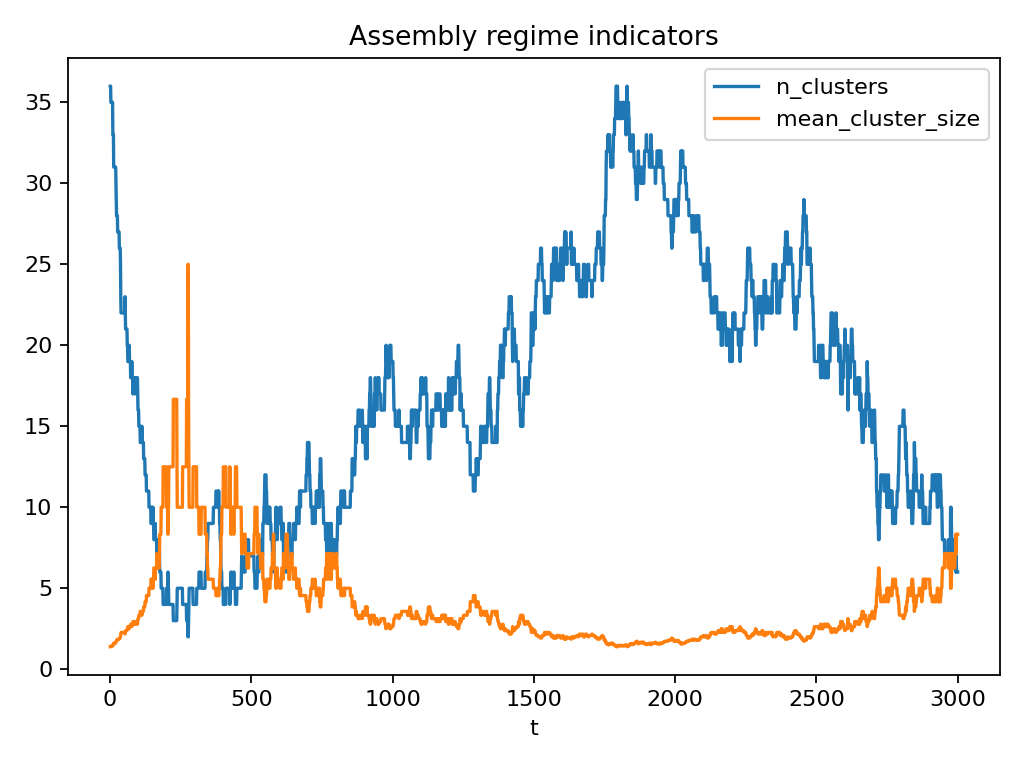
\includegraphics[width=0.92\linewidth]{figures/plot_clusters_Hprime_seed0.png}
  \caption{\textbf{(H$'$) Assembly regime indicators.} $n_{\text{clusters}}(t)$ spans a wide range with sustained fragmentation,
  while mean cluster size remains low for long intervals. This is consistent with repeated reconfiguration cycles in the assembly graph.}
  \label{fig:Hp_clusters}
\end{figure}

\begin{figure}[t]
  \centering
  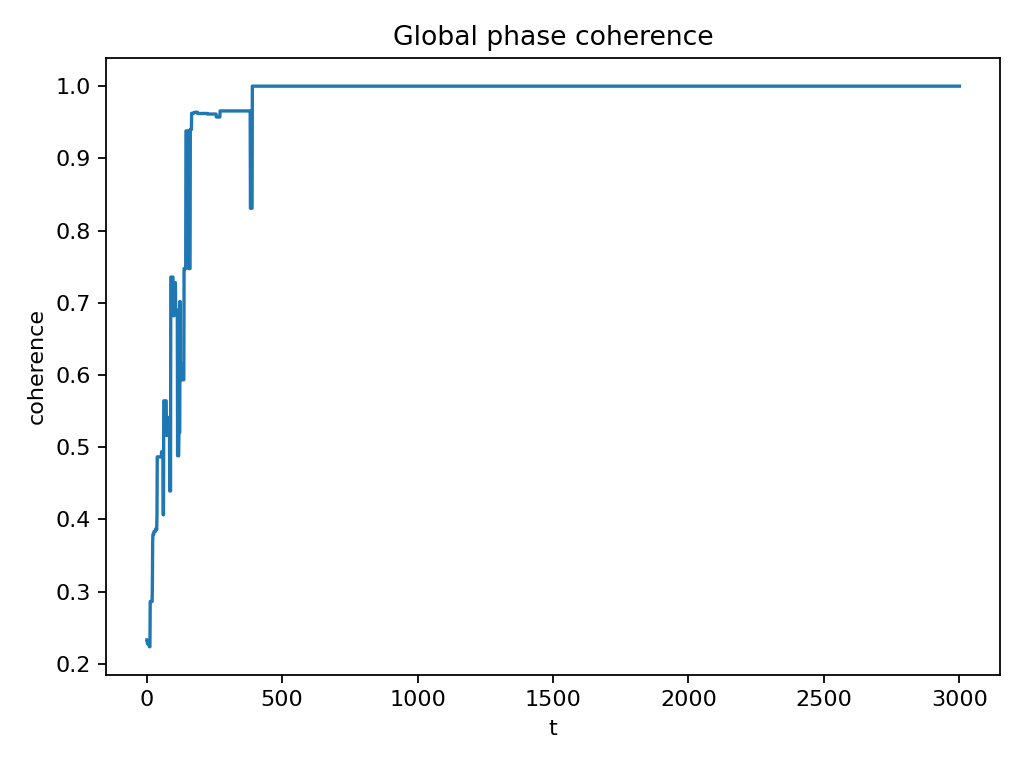
\includegraphics[width=0.92\linewidth]{figures/plot_coherence_Hprime_seed0.png}
  \caption{\textbf{(H$'$) Global phase coherence.} Coherence still reaches $1$ and remains locked.
  This indicates that phase synchronization is absorbing under deterministic identical oscillators: once phases become equal,
  they remain equal even if the population later detaches into multiple components.}
  \label{fig:Hp_coherence}
\end{figure}

\begin{figure}[t]
  \centering
  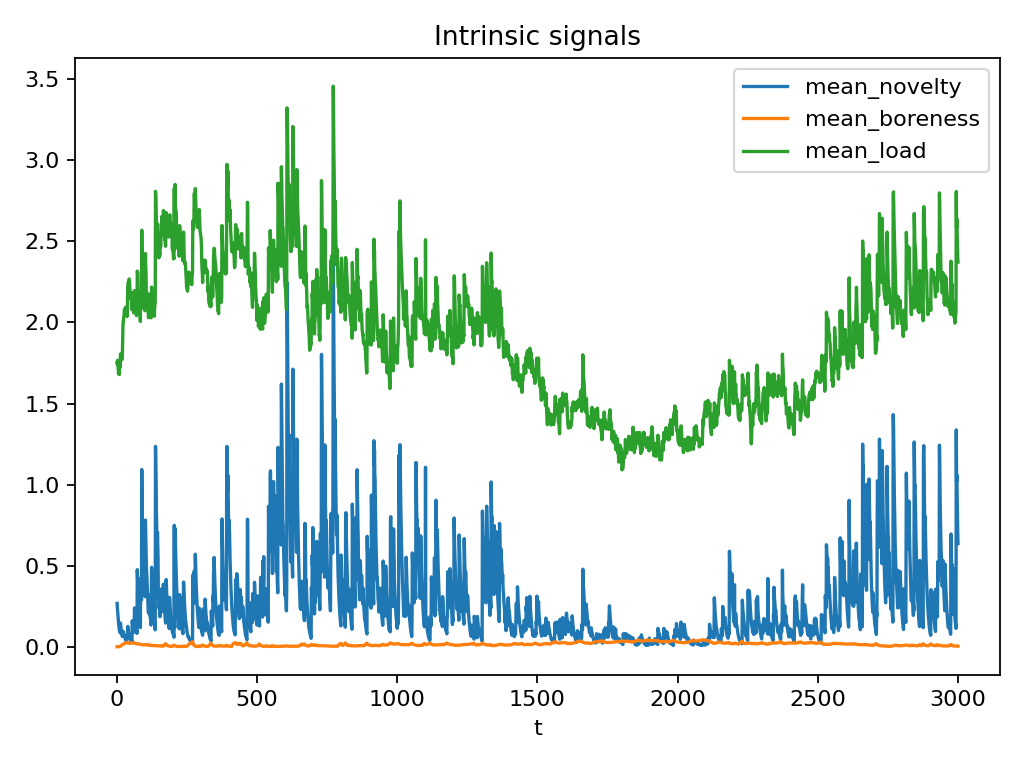
\includegraphics[width=0.92\linewidth]{figures/plot_intrinsic_Hprime_seed0.png}
  \caption{\textbf{(H$'$) Intrinsic signals.} Load varies with interaction intensity; novelty exhibits recurrent spikes during reconfiguration.
  Boreness remains small at the current plotting scale (consistent with an $\mathcal{O}(\eta)$ equilibrium under low novelty).}
  \label{fig:Hp_intrinsic}
\end{figure}

\section{H$''$ plan: heterogeneous natural frequencies to make coherence regime-sensitive}
To avoid coherence becoming an absorbing indicator, we introduce a small per-agent heterogeneity in oscillator natural frequencies:
\[
\omega_{0,k} \sim \mathcal{N}(\omega_0,\sigma_{\omega}^2).
\]
Operationally, we keep merge-triggered synchronization (hard or soft), but after detachments each component's phases will drift due to slightly
different $\omega_{0,k}$, allowing coherence to decrease and track regime changes.
This modification is minimal, preserves the embodied semantics, and provides an interpretable control parameter $\sigma_{\omega}$.

\paragraph{Implementation note.}
The code should store a fixed $\omega_{0,k}$ per agent at initialization (seed-controlled), log it for reproducibility, and update phases by
$\varph_k(t+\Delta t)=\varph_k(t)+\omega_{0,k}\Delta t \pmod{1}$.

\section{References}
\begin{thebibliography}{10}

\bibitem{canonne_garnier_mcm2011}
Cl{\'e}ment Canonne and Nicolas Garnier.
\newblock A Model for Collective Free Improvisation.
\newblock In \emph{Mathematics and Computation in Music (MCM), Third International Conference},
  \emph{Lecture Notes in Computer Science}, vol.~6726, pp.~29--41. Springer, 2011.
\newblock DOI: \href{https://doi.org/10.1007/978-3-642-21590-2_3}{10.1007/978-3-642-21590-2\_3}.

\bibitem{lucas_acsos2024_embodied}
Pedro Lucas, Alexander Szorkovszky, Stefano Fasciani, and Kyrre Glette.
\newblock Self-Assembly and Synchronization: Crafting Music with Multi-Agent Embodied Oscillators.
\newblock In \emph{Proceedings of the IEEE International Conference on Autonomic Computing and Self-Organizing Systems (ACSOS)},
  pp.~145--150. IEEE, 2024.
\newblock DOI: \href{https://doi.org/10.1109/ACSOS61780.2024.00034}{10.1109/ACSOS61780.2024.00034}.

\end{thebibliography}

\end{document}